\section{Bind DNS Server}

\subsection{Installation}
Installation of the \emph{Bind DNS} is done easily with Ubuntu's package manager \emph{apt}. The following command does the job of installation:

\texttt{sudo apt-get install bind9}

To check the installation use a CLI tool called \emph{dig}. If this is not available, install it in the same manner as \emph{apt}, with the command:

\texttt{sudo apt-get install dnsutil}

When \emph{dig} is available, check the installation of \emph{Bind}. This is done by checking the loop-back interface on \emph{127.0.0.1}.

\texttt{dig -x 127.0.0.1}

Which, if successful, should give an output looking like:

\texttt{;; Query time: 3 msec}\\
\texttt{;; SERVER: 127.0.1.1\#53(127.0.1.1)}

\subsection{Configuration}
The \emph{Bind} server can be configured in a wide variety of ways, but in this report, the focus will be configuring it as a \emph{Caching name server} and a \emph{Forwarder}. Configuration files are located at \emph{/etc/bind}, with the main configuration files being:

\emph{/etc/bind/named.conf.local}\\
\emph{/etc/bind/named.conf.options}\\
\emph{/etc/bind/named.conf}\\

\subsubsection{Caching name server}
Using \emph{Bind} as a \emph{Caching name server} reduces DNS query time, since the server stores answers to name queries, and only forwards the query if it does not already know the answer.
By default caching is enabled on the \emph{Bind} server. To test this functionality a previously unvisited site is checked with \emph{dig}, two times.

\begin{figure}[ht!]
\centering
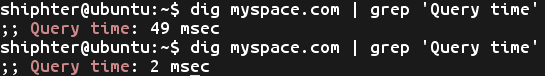
\includegraphics[width=90mm]{img/dig_caching_querytime.png}
\caption{Caching name server improving query time}
\label{dig_caching_querytime}
\end{figure}

As expected it is found, see figure \ref{dig_caching_querytime}, that the caching functionality vastly improves query time.

\subsubsection{Forwarding} 


\subsection{Analyzing public DNS servers}
In the quest of finding the best public DNS server, Google's tool \emph{namebench} is used. The results looks as follows:


\begin{figure}[ht!]
\centering
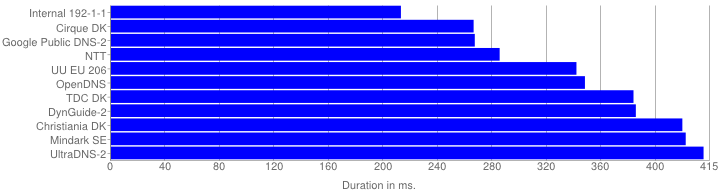
\includegraphics[width=150mm]{img/namebench_meantime_response_chart.png}
\caption{Google Namebench - Meantime response}
\label{namebench_meantime_response_chart}
\end{figure}

\begin{figure}[ht!]
\centering
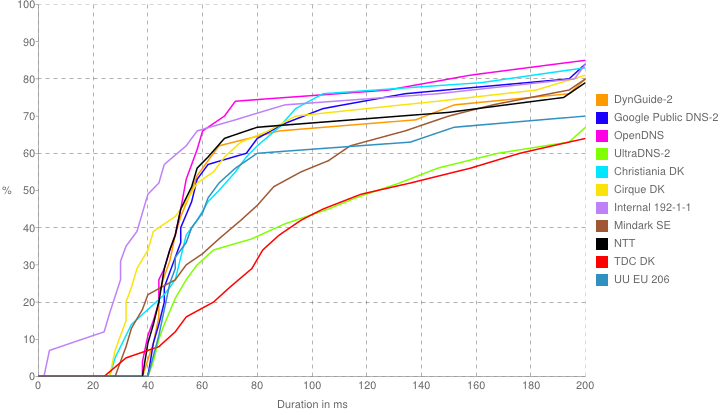
\includegraphics[width=150mm]{img/namebench_response_distro.png}
\caption{Google Namebench - Response distribution the first 200 ms}
\label{namebench_response_distro}
\end{figure}

From this, we find Google to be the best alternative, since this is both public, fast and secure.
